\documentclass[twocolumn]{article}
\usepackage[utf8]{inputenc}

\usepackage{tikz}
\usetikzlibrary{external}
\usetikzlibrary{shapes}
\usetikzlibrary{fit}

\usepackage{etoolbox} %for if empty functionality
\usepackage{leftidx}
\usepackage{ifthen}

\newcounter{a}
\newcounter{b}



\usepackage{braket}

\usepackage{subcaption} % Subfigure environment 
\usepackage{gensymb}

\usepackage{amsmath} % Mathematical symbols
\usepackage{amssymb} % Symbols

\usepackage{caption}% Captions onder figuur gecentreerd
%\usepackage[toc,page]{appendix}
\usepackage{subcaption} % Subfigure environment 
\usepackage{float}

\usepackage{etoolbox} %for if empty functionality

\usepackage{ifthen}

%break long urls at a - and not only at . or /
\usepackage{url}
\def\UrlBreaks{\do\/\do-}
\usepackage{breakurl}
\usepackage[hidelinks,breaklinks]{hyperref}

\usepackage{verbatim}
\usepackage{cleveref}
\usepackage{amsfonts}
\usepackage{mathtools}

\usepackage{braket}
\usepackage{pdfpages}

\title{Cluster Expansion of Thermal States using Tensor
Networks}
\author{David Devoogdt}
\date{Academic year 2020-2021}


\begin{document}

\tikzset{add reference/.style={insert path={%
                    coordinate [pos=0,xshift=-0.5\pgflinewidth,yshift=-0.5\pgflinewidth] (#1 south west)
                    coordinate [pos=1,xshift=0.5\pgflinewidth,yshift=0.5\pgflinewidth]   (#1 north east)
                    coordinate [pos=.5] (#1 center)
                    (#1 south west |- #1 north east)     coordinate (#1 north west)
                    (#1 center     |- #1 north east)     coordinate (#1 north)
                    (#1 center     |- #1 south west)     coordinate (#1 south)
                    (#1 south west -| #1 north east)     coordinate (#1 south east)
                    (#1 center     -| #1 south west)     coordinate (#1 west)
                    (#1 center     -| #1 north east)     coordinate (#1 east)
                }}}
%\def\temp{#1}\ifx\temp\empty
%  <EMPTY>%
%\else
%  <NON EMPTY>%
%\fi




%use first argument is numbers of O's, second the labels, can be empty
%\mpo{3}{ {0,1,2,3,4} }

\newcommand{\combineTikz}[3]{
    \begin{tikzpicture}[baseline={0-0.5*height("$=$")}]
        \node (AA) at (0,0)  { #1   };
        \node (AB) at ( {#3} ,0)  {  #2  };
    \end{tikzpicture}
}


\newcommand{\mpo}[6]  { \begin{tikzpicture}[baseline={0-0.5*height("$=$")}]
        %\def \NNodes {#1}
        %\def \NodeName {#2}          
        %\def \NameUp   {#3} 
        %\def \NameDown  {#4}	

        \def \legLength {0.6}
        \def \radius {0.3}

        \pgfmathsetmacro{\step}{2*\radius+\legLength}
        \pgfmathsetmacro{\legpos}{\radius+\legLength}

        \pgfmathsetmacro{\Nmax}{#1-1}

        \foreach \N in {0,..., \Nmax }{
                \pgfmathsetmacro{\p}{\N*\step}

                % up and down labels
                \def\temp{#3}\ifx\temp\empty
                    \def \labelUp {}
                \else
                    \pgfmathsetmacro{\labelUp}{  {#3}[\N]  }
                \fi

                \def\tempp{#4}\ifx\tempp\empty
                    \def \labeldown {}
                \else
                    \pgfmathsetmacro{\labeldown}{  {#4}[\N]  }
                \fi


                \def\aab{#5}\ifx\aab\empty
                    \def \dotssite {0}
                \else
                    \pgfmathsetmacro{\dotssite}{  {#5}[\N]  }
                \fi

                \ifthenelse{\dotssite = 0}{

                    \def\aac{#6}\ifx\aac\empty
                        \def \nname {O}
                    \else
                        \pgfmathsetmacro{\nname}{  {#6}[\N]  }
                    \fi



                    \node[circle,draw, radius=\radius] (O\N) at (\p,0) {\nname};


                    \node[] (Ou\N) at (\p, \legpos ) { \labelUp };


                    \node[] (Od\N) at (\p,-\legpos) {\labeldown};


                    \draw (O\N) -- (Ou\N);
                    \draw (O\N) -- (Od\N);
                }{
                    \node[circle] (O\N) at (\p,0) { $\cdots$ };


                }


            }

        \ifthenelse{  #1  =1  }{}{
            \foreach \N in {1,...,\Nmax }{
                    \pgfmathsetmacro{\M}{\N-1}
                    \pgfmathsetmacro{\label}{ {#2}[\N]  }
                    %\pgfmathsetmacro{\label}{ 5}

                    \draw (O\M) --  node[above]  {\label} (O\N);
                }
        }

        \pgfmathsetmacro{\labelo}{ {#2}[0]}
        \pgfmathsetmacro{\labeli}{  {#2}[\Nmax+1]}

        \node (N0) at (-\legpos,0) {};
        \draw (N0) -- node[above] {\labelo} (O0);

        \pgfmathsetmacro{\endpos}{\step*\Nmax+\legpos}

        \node (Ne) at (\endpos,0) {};
        \draw (Ne) -- node[above] {\labeli} (O\Nmax);

        %\draw (O0) --  node[above] {1} (O1);


    \end{tikzpicture}}

\newcommand{\expH}[5]{ \begin{tikzpicture}[baseline={0-0.5*height("$=$")}]

        \def \NNodes {#1};


        \def\aaa{#2}\ifx\aaa\empty
            \def \text { $e^{-\beta \hat{H}_{\NNodes} }$ }
        \else
            \def \text {#2}
        \fi

        \pgfmathwidth{ "\text" }
        \def \textwidth { \pgfmathresult }


        %\pgfmathsetmacro{\text}{width(\text)}

        \def \legLength {0.6}
        \def \radius {0.3} %fix to fit text inside for size 1
        \def \boxHeight {0.4};

        \pgfmathsetmacro{\step}{2*\radius+\legLength}
        \pgfmathsetmacro{\legpos}{\radius+\legLength}
        \pgfmathsetmacro{\dotpos}{\boxHeight+\legLength/2}

        \pgfmathsetmacro{\Nmax}{\NNodes -1}



        \pgfmathsetmacro{\boxsize}{ max ( \textwidth/1cm , \step*\Nmax )   + \radius}

        %\pgfmathsetmacro{\boxsize}{ 5  )}
        %\pgfmathsetlength{\boxsize}{ max( \textwidth,  \boxsize1  )}



        %            \ifthenelse{#1=1}{
        %                \def \left {-0.6}
        %                \def \right {0.6}
        %            }{
        \def \left {-\radius}
        \def \right {\boxsize}
        %            }

        \draw (\left,- \boxHeight ) rectangle (\right, \boxHeight ) [add reference =H] ;


        \node  at (H center) { \text };

        \foreach \N in {0,..., \Nmax }{
                \pgfmathsetmacro{\p}{\N*\step}

                % up and down labels
                \def\temp{#3}\ifx\temp\empty
                    \def \labelUp {}
                \else
                    \pgfmathsetmacro{\labelUp}{  {#3}[\N]  }
                \fi

                \def\tempp{#4}\ifx\tempp\empty
                    \def \labeldown {}
                \else
                    \pgfmathsetmacro{\labeldown}{  {#4}[\N]  }
                \fi


                \node[] (O\N) at (\p,0) {};


                \ifthenelse{ \equal{\labelUp}{...}  }{
                    \node[] (Ou\N) at (\p, \dotpos ) {\labelUp};
                }{
                    \node[] (Ou\N) at (\p, \legpos ) {\labelUp};
                    \draw (Ou\N) --  (Ou\N  |- H north);
                }


                \ifthenelse{ \equal{\labeldown}{...}  }{
                    \node[] (Od\N) at (\p,-\dotpos ) {\labeldown};
                }{
                    \node[] (Od\N) at (\p,-\legpos) {\labeldown};
                    \draw (Od\N) --  (Od\N  |- H south);
                }
            }

        \def\tempt{#5}\ifx\tempt\empty

        \else
            \pgfmathsetmacro{\labelo}{ {#5}[0] }
            \pgfmathsetmacro{\labeli}{  {#5}[1] }

            \pgfmathsetmacro{\leftleg}{  \left - \legLength }
            \pgfmathsetmacro{\rightleg}{  \right + \legLength }

            \node (N0) at (\leftleg,0) {\labelo};
            \draw (N0) -- ( N0  -| H west);

            \node (Ne) at (\rightleg,0) {\labeli};
            \draw (Ne) --  ( Ne  -| H east);
        \fi


    \end{tikzpicture} }



\maketitle

\begin{abstract}
    Simulating many-body quantum systems is one of the challenges faced by modern Physics. One particular problem is computing the operator $e^{-\beta \hat{H}}$, which is used to compute the partition function of a quantum model.  This function is needed to make prediction about the macroscopic behaviour of quantum systems. Of particular interest are the phase transitions. The dissertation introduces the rich field of tensor networks as a method to perform these calculations. The physics of strongly correlated matter is discussed. The main contribution of this work, the novel cluster expansions, are described, together with the computational tools to solve the equations efficiently. The results are promising. Large imaginary time steps can be taken. Calculating of the phase transition of transversal field Ising model in 2D produces results that can challenge recent developments in literature.

\end{abstract}

\section{Introduction}

\section{Tensor Networks}

Matrix Product States (MPS) form an ansatz to describe the
\begin{equation}
    \ket{\Psi} = \sum_{i_1 i_2 \cdots i_n } C^{i_1 i_2 \cdots i_n} \ket{i_1} \otimes \ket{i_2} \otimes \cdots \otimes \ket{i_n}
\end{equation}
The tensor C needs $d^n$ numbers to describe the full wave function. In uniform MPS, the tensor $ C^{i_1 i_2 \cdots i_n}$ is subdivided into the product of n tensors $C$ and a matrix $M$ that contains the boundary conditions
\begin{equation} \label{c_split}
    C^{i_1 i_2 \cdots i_n} = Tr( C^{i_1} C^{i_2} \cdots C^{i_n} M  ).
\end{equation}
If M is the identity matrix, the chain is closed cyclically. Tensor networks are typically denoted in their graphical form (see \cref{tab:grafical_not}). External lines denote free indices, connected lines implies a summation over the shared line, analogous to matrix multiplication.
\begin{table}[]
    \centering
    \caption{Caption}
    \begin{tabular}{l|l|l}
        conventional            & Einstein                & tensor notation           \\
        \hline
        $\Vec{x}$               & $x_{\alpha}$            &

        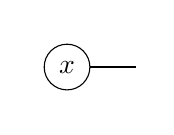
\begin{tikzpicture}[baseline=({N2.base}) ]
            \clip (-0.5,-0.5) rectangle (1,0.5);
            \node[circle, draw] (N2) at (0,0) {$x$};
            \node[] (N1) at (1,0) {};
            \draw  (N1) -- (N2) ;
        \end{tikzpicture}                                                     \\
        M                       & $M_{\alpha \beta}$      & 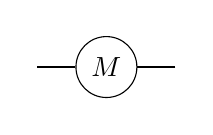
\begin{tikzpicture}[baseline={0cm-0.5*height("$=$")} ]
            \clip (-1,-0.5) rectangle (1,0.5);

            \node[circle, draw] (N2) at (0,0) {$M$};
            \node[] (N0) at (-1,0) {};
            \node[] (N1) at (1,0) {};

            \draw  (N1) -- (N2) ;
            \draw  (N0) -- (N2) ;

        \end{tikzpicture} \\

        $\Vec{x} \cdot \Vec{y}$ & $x_{\alpha} y_{\alpha}$ & 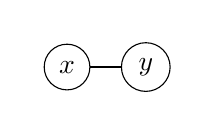
\begin{tikzpicture}[baseline=({N2.base}) ]
            \clip (-0.5,-0.5) rectangle (1.5,0.5);
            \node[circle, draw] (N2) at (0,0) {$x$};
            \node[circle, draw] (N1) at (1,0) {$y$};
            \draw  (N1) -- (N2) ;
        \end{tikzpicture} \\
    \end{tabular}

    \label{tab:grafical_not}
\end{table}
\Cref{c_split} is in this graphical notation becomes
\begin{equation}\label{eq:general_mps}
    \mpo{5}{{"Tr",,,,,}}{{"$i_1$","$i_2$",,"$i_n$","-"}}{{"-","-",,"-","-"}}{{0,0,1,0,0}}{{"C", "C",,"C","M" }}.
\end{equation}
An MPS has 2 dimension, the physical dimnsion of the particles $d = dim \left( \ket{i_2}  \right)$ and the dimension $\chi$ of the bonds between the tensors. The cluster expansion will rely on "virtual levels". This is the division of the MPS in blocks, analogous to dividing a matrix into block matrices. Every virtual level has its own associated dimension
\subsection{MPO}
A matrix procuct operator (MPO), is similar to an MPS but has 2 physical legs $i$ and $j$. The following compact notation is used in this paper
\begin{equation}
    \mpo{1}{ {0,0}  }{ {"$i$",}  }{ {"$j$",}}{}{{"",}} = \mpob{1}{ {0,0}  }{ {"$i$",}  }{ {"$j$",}}{}{{"",}}.
\end{equation}
This is the MPO with virtual level 0 and physical indices $i$ and $j$, which will both be omitted. Non-zero virtual indices are shown, and summation over virtual level is implied. Summation over shared virtual bond 1 on 2 neighbouring sites is denoted as
\begin{equation}
    \mpob{2}{ {0,1,0}  }{ {"$i_1$","$i_2$"}  }{ {"$j_1$","$j_1$",}}{}{{"",}}.
\end{equation}
While contraction over all possible virtual levels on 3 sites is denoted by
\begin{equation} \label{PEPO_3}
    \mpob{3}{ {0,,,0}  }{}{}{}{{"",,}} .
\end{equation}

\section{Strongly correlated matter}

\subsection{Transversal Ising}

\begin{figure}[h!]
    \center
    \includegraphics[width=\linewidth]{../Figuren/phsyics/2disingphase.png}
    \caption{Phase diagram for 2D transversal Ising model. Figure taken from \cite{Hesselmann2016}.}
    \label{2dtisingphasediag}
\end{figure}

\subsection{Criticality}

\subsection{operator exponentials}

\subsection{TN contraction}

\section{Cluster Expansion}

The novel method to construct a PEPO $e^{-\beta \hat{H}}$ with cluster expansions. An example is given by \cref{PEPO_3}.  This was first introduced in \cite{Vanhecke2021}. The goal is capture the exponential of the Hamiltonian operator $\hat{H}$
\begin{equation}
    \hat{H} = \left (  \sum_{<i j>} H^i_2 H^j_2 + \sum_i H^i_1 \right )
\end{equation}
This Hamiltonian consists of 1 and 2 site operators. Of course more general Hamiltonians can also be used. The notation for the contraction of the tensor network will also be used to denote the Hamiltonian evaluated on the given geometry
\begin{alignat}{3}
    H \left( \mpob{3}{ {0,,,0}  }{}{}{}{{"",,}} \right ) = & H_1 &  & \otimes 1   &  & \otimes 1  \nonumber  \\
    +                                                      & 1   &  & \otimes H_1 &  & \otimes 1 \nonumber   \\
    +                                                      & 1   &  & \otimes 1   &  & \otimes H_1 \nonumber \\
    +                                                      & H_2 &  & \otimes H_2 &  & \otimes 1   \nonumber \\
    +                                                      & 1   &  & \otimes H_2 &  & \otimes H_2 \nonumber \\.
\end{alignat}

\subsection{Idea}

The main idea is to make an extensive expansion by adding blocks which solve the model exactly on a local patch. Crucially, the expansion is not in the inverse temperature $\beta$ but in the size of the patches. The local patches are separated by a virtual level 0 bond. To make this somewhat more precise, the first steps of the expansion are shown here. The smallest patch, i.e. 1 site,  encodes the exponential of that Hamiltonian
\begin{equation}
    \mpob{1}{ {0,0}  }{}{}{}{{"",}} = \exp \left( -\beta H(\mpob{1}{}{}{}{}{{"",}})   \right).
\end{equation}
If there were no 2 site interactions, this already captures the full diagonalisation. Of course, such a model wouldn't be useful. The next step is to introduce 2 site interactions, where the one site interactions are subtracted from the diagonalised Hamiltonian.
\begin{equation} \label{eq:lev1}
    \begin{split}
        \mpob{2}{ {0,1,0}  }{}{}{}{{"",}}  = \exp -\beta H( & \mpob{2}{ {,,} }{}{}{}{{"",}})  \\
        - &\mpob{2}{ {0,0,0}  }{}{}{}{{"",}}
    \end{split}
\end{equation}
Contraction of larger network lead to many terms, such as
\begin{equation}
    \mpob{10}{ {0,1,0,0,0,1,0,1,0,0,1,0}  }{}{}{}{{"","","","","","","","","","","",}} .
\end{equation}
The beauty of this lays in the fact that disconnected regions(regions separated by level 0) combine in exactly the right way to capture the terms appearing in the series expansion of the exact tensor exponential. \cite{Vanhecke2021} Only the terms of the exponential which acts on 3 or more neighbouring sites at once, are not accounted for.

Notice that in \cref{eq:lev1}, 2 new blocks are introduced. The dimension of virtual level 1 needs to be $d^2$, with d the dimension of physical level. Although different possible constructions, already differ in the next step, one more step is added to make te construction and notation clear.
\begin{equation}\label{constr:intro:gen}
    \begin{split}
        \mpob{3}{ {0,1,1,0}  }{}{}{}{{,,,}}  = \exp  -\beta H( &\mpob{3}{ {,,,} }{}{}{}{{,,}})  \\
        - \;&\mpob{3}{ {0,0,0,0}  }{}{}{}{{,,,}}\\
        - \; &\mpob{3}{ {0,1,0,0}  }{}{}{}{{,,,}}\\
        - \; &\mpob{3}{ {0,0,1,0}  }{}{}{}{{,,,}}\\
        =\exp  -\beta H( &\mpob{3}{ {,,,} }{}{}{}{{,,}})\\
        - \; &\mpob{3}{ {,,,}  }{}{}{}{{,,,}}\\
    \end{split}
\end{equation}
This is called an cluster expansion of order 3, because there are 3 connected sites solved exactly. The right-hand side of \cref{constr:intro:gen} can be ommited, as it is just evaluating the exponentiated Hamiltonian on the same geometry as the left hand side and substructing all possible contractions of the blocks which were added previously. This very compact notation will be able to capture the essence of the different constructions. Because it is important for the remainder of the chapter, it is stressed that for an equation similar to
\begin{equation}
    \boxed{\mpob{3}{ {0,1,1,0}  }{}{}{}{{,,,}} },
\end{equation}
the right-hand side of \cref{constr:intro:gen} is implied. In the following section, different types will be discussed. For every chain lenght, a new block is defined. This could be done in numerous ways. The different types will be discussed in the next sections.

\subsection{1D}
\subsubsection{Type A}
\begin{subequations}
    \begin{align}
         & \mpob{1}{ {,}  }{}{}{}{{,,}}                     \\
         & \mpob{2}{ {,"1",}  }{}{}{}{{,,}}                 \\
         & \mpob{3}{ {,"1","1",}  }{}{}{}{{,,,}}            \\
         & \mpob{4}{ {,"1","2","3",}  }{}{}{}{{,,,,,}}      \\
         & \mpob{5}{ {,"1","2","3","4",}  }{}{}{}{{,,,,,}}.
    \end{align}
\end{subequations}
\subsubsection{Type E}
\begin{subequations}
    \begin{align}
         & \mpob{1}{ {,}  }{}{}{}{{,,}}                      \\
         & \mpob{2}{ {,"1",}  }{}{}{}{{,,}}                  \\
         & \mpob{3}{ {,"1","1'",}  }{}{}{}{{,,,}}            \\
         & \mpob{4}{ {,"1","2","1'",}  }{}{}{}{{,,,,,}}      \\
         & \mpob{5}{ {,"1","2","2'","1'",}  }{}{}{}{{,,,,,}}
    \end{align}
\end{subequations}

\subsubsection{Type F}

\begin{subequations}
    \begin{align}
         & \mpob{1}{ {,}  }{}{}{}{{,,}}                                          \\
         & \mpob{2}{ {,"1'",}  }{}{}{}{{,,}}+  \mpob{2}{ {,"1'",}  }{}{}{}{{,,}} \\
         & \mpob{3}{ {,"1","1",}  }{}{}{}{{,,,}}                                 \\
         & \mpob{4}{ {,"1","2","1",}  }{}{}{}{{,,,,,}} \; +  \nonumber           \\
         & \mpob{4}{ {,"1","2'","1",}  }{}{}{}{{,,,,,}}                          \\
         & \mpob{5}{ {,"1","2","2","1",}  }{}{}{}{{,,,,,}}
    \end{align}
\end{subequations}

\subsection{2D}
\subsubsection{Linear}

\begin{equation}
    \mpob{1}{ {,}  }{}{}{}{{,,}} = \vcenter{ \hbox{ \pepob{4}{3}{{
                        "-","-","-",
                        "-","0","0",
                        "-","-","-"}}{{
                        "-","-",
                        "-","-",
                        "0","0",
                        "-","-"}}{{
                        1,1,4,1,
                        1,4,12,4,
                        1,1,4,1}} }}
\end{equation}

\begin{equation}\label{2dblocksorder2}
    \pepob{2}{2}{{"1",,}}{{,,}}{{0,0,1,1}}  \pepob{2}{2}{{,,}}{{"1",,}}{{0,1,0,1}}
\end{equation}

\begin{equation}
    \pepob{2}{2}{{"1","1",}}{{"1","1",}}{{0,0,0,1}} \;
    \pepob{3}{2}{{"1","1","1","1"}}{{"1","1","1","1"}}{{0,0,0,1,1,1}}
\end{equation}

and rotations

\begin{equation}
    \pepob{3}{2}{{"1","1","1","1"}}{{"1","1","1","1"}}{{0,0,0,1,0,1}} \;   \pepob{3}{3}{{"1","1","1","1","1","1",}}{{"1","1","1","1","1","1",}}{{1,0,1,0,0,0,1,0,1}}
\end{equation}

\subsubsection{Nonlinear}

\begin{equation}
    {\pepob{2}{2}{{"","",}}{{"","",}}{{0,0,0,0}}}
\end{equation}

\subsection{Solvers}

\def \pepoat {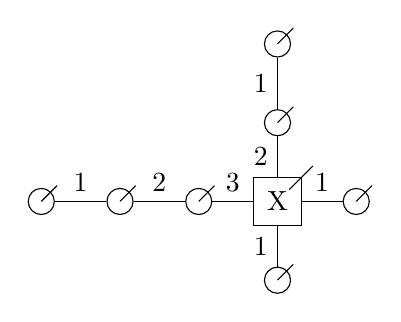
\begin{tikzpicture}[baseline=0.5]

        \def \legLength { 0.8}
        \def \radius {0.1}

        \pgfmathsetmacro{\step}{2*\radius+ \legLength} % 1
        \pgfmathsetmacro{\legpos}{\radius+\legLength} %0.9

        \node[draw,minimum size=0.6cm] (O0) at (0,0) {X};
        \draw (0.15,0.15) -- ++(0.3,0.3);

        \node[draw, circle,radius=\radius] (L1) at (-1,0) {};
        \node[draw, circle,radius=\radius] (L2) at (-2,0) {};
        \node[draw, circle,radius=\radius] (L3) at (-3,0) {};

        \node[draw, circle,radius=\radius] (U1) at (0,1) {};
        \node[draw, circle,radius=\radius] (U2) at (0,2) {};

        \node[draw, circle,radius=\radius] (D1) at (0,-1) {};

        \node[draw, circle,radius=\radius] (R1) at (1,0) {};

        \draw (O0) -- node [above] {3}  (L1);
        \draw (L2) -- node [above] {2}  (L1);
        \draw (L2) -- node [above] {1}  (L3);

        \draw (O0) -- node [left] {2}  (U1);
        \draw (U2) -- node [left] {1}  (U1);

        \draw (O0) -- node [above] {1}  (R1);

        \draw (O0) --  node [left] {1} (D1);

        \draw (L1.center) -- ++(0.2,0.2);
        \draw (L2.center) -- ++(0.2,0.2);
        \draw (L3.center) -- ++(0.2,0.2);
        \draw (U1.center) -- ++(0.2,0.2);
        \draw (U2.center) -- ++(0.2,0.2);
        \draw (R1.center) -- ++(0.2,0.2);
        \draw (D1.center) -- ++(0.2,0.2);

    \end{tikzpicture}}

\def \blockat {  \begin{tikzpicture}[baseline=0.5]

        \def \legLength { 0.8}
        \def \radius {0.1}

        \pgfmathsetmacro{\step}{2*\radius+ \legLength} % 1
        \pgfmathsetmacro{\legpos}{\radius+\legLength} %0.9

        %\node[draw=none] (O0) at (0,0) {};
        \node[draw=none,minimum size=0.6cm] (O0) at (0,0) {B};
        \draw (0.15,0.15) -- ++(0.3,0.3);

        \node[draw=none] (L1) at (-1,0) {};
        \node[draw=none] (L2) at (-2,0) {};
        \node[draw=none] (L3) at (-3,0) {};

        \node[draw=none] (U1) at (0,1) {};
        \node[draw=none] (U2) at (0,2) {};

        \node[draw=none] (D1) at (0,-1) {};

        \node[draw=none] (R1) at (1,0) {};

        %\draw (O0.center) -- ++(0.45,0.45);
        \draw (L1.center) -- ++(0.2,0.2);
        \draw (L2.center) -- ++(0.2,0.2);
        \draw (L3.center) -- ++(0.2,0.2);
        \draw (U1.center) -- ++(0.2,0.2);
        \draw (U2.center) -- ++(0.2,0.2);
        \draw (R1.center) -- ++(0.2,0.2);
        \draw (D1.center) -- ++(0.2,0.2);

        \draw (-3.3,0.3)--(-0.3,0.3) -- (-0.3,2.3)--(0.3,2.3)
        -- (0.3,0.3) -- (1.3,0.3) -- (1.3,-0.3) -- (0.3,-0.3)
        -- (0.3,-1.3) -- (-0.3, -1.3) -- (-0.3,-0.3) -- (-3.3,-0.3) -- cycle;

    \end{tikzpicture}}

\def \pepobt {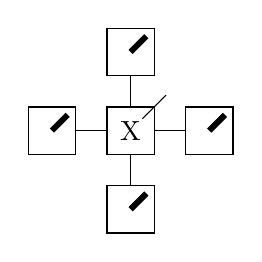
\begin{tikzpicture}[baseline=0.5]

        \def \legLength { 0.8}
        \def \radius {0.1}

        \pgfmathsetmacro{\step}{2*\radius+ \legLength} % 1
        \pgfmathsetmacro{\legpos}{\radius+\legLength} %0.9

        %\node[draw, circle, radius=\radius] (O0) at (0,0) {};
        \node[draw,minimum size=0.6cm] (O0) at (0,0) {X};
        \draw (0.15,0.15) -- ++(0.3,0.3);

        \node[draw, minimum size=0.6cm] (L1) at (-1,0) {};
        \node[draw, minimum size=0.6cm] (U1) at (0,1) {};
        \node[draw, minimum size=0.6cm] (D1) at (0,-1) {};
        \node[draw, minimum size=0.6cm] (R1) at (1,0) {};

        \draw (O0) -- (L1);
        \draw (O0) -- (U1);
        \draw (O0) -- (R1);
        \draw (O0) -- (D1);

        %\draw(O0.center) -- ++(0.2,0.2);
        \draw[line width=0.75mm]  (L1.center) -- ++(0.2,0.2);
        \draw[line width=0.75mm] (U1.center) -- ++(0.2,0.2);
        \draw[line width=0.75mm] (R1.center) -- ++(0.2,0.2);
        \draw[line width=0.75mm] (D1.center) -- ++(0.2,0.2);

    \end{tikzpicture} }

\def \blockbt {   \begin{tikzpicture}[baseline=0.5]

        \def \legLength { 0.8}
        \def \radius {0.1}

        \pgfmathsetmacro{\step}{2*\radius+ \legLength} % 1
        \pgfmathsetmacro{\legpos}{\radius+\legLength} %0.9

        %\node[draw=none] (O0) at (0,0) {};
        \node[draw=none,minimum size=0.6cm] (O0) at (0,0) {B};
        \draw (0.15,0.15) -- ++(0.3,0.3);

        \node[draw=none] (L1) at (-1,0) {};
        \node[draw=none] (L2) at (-2,0) {};
        \node[draw=none] (L3) at (-3,0) {};

        \node[draw=none] (U1) at (0,1) {};
        \node[draw=none] (U2) at (0,2) {};

        \node[draw=none] (D1) at (0,-1) {};

        \node[draw=none] (R1) at (1,0) {};

        %\draw (O0.center) -- ++(0.45,0.45);
        \draw[line width=0.75mm] (L3.center) -- ++(0.2,0.2);
        \draw[line width=0.75mm] (U2.center) -- ++(0.2,0.2);
        \draw[line width=0.75mm] (R1.center) -- ++(0.2,0.2);
        \draw[line width=0.75mm] (D1.center) -- ++(0.2,0.2);

        \draw (-3.3,0.3)--(-0.3,0.3) -- (-0.3,2.3)--(0.3,2.3)
        -- (0.3,0.3) -- (1.3,0.3) -- (1.3,-0.3) -- (0.3,-0.3)
        -- (0.3,-1.3) -- (-0.3, -1.3) -- (-0.3,-0.3) -- (-3.3,-0.3) -- cycle;

    \end{tikzpicture} }

\def \pepoct { 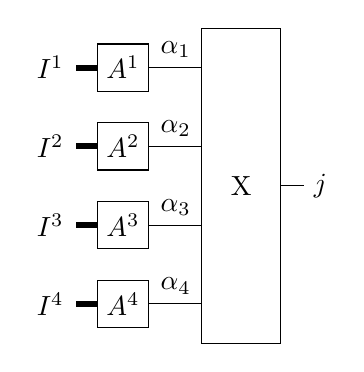
\begin{tikzpicture}[baseline=0.5]
        \draw (0,2.5)-- (0,-1.5) -- (1,-1.5)-- (1,2.5) -- cycle;

        \node[draw=none] (x)  at (0.5,0.5) {X};

        \node[draw, minimum size=0.6cm] (n1)  at (-1,2) {$A^1$};
        \node[draw, minimum size=0.6cm] (n2)  at (-1,1) {$A^2$};
        \node[draw, minimum size=0.6cm] (n3)  at (-1,0) {$A^3$};
        \node[draw, minimum size=0.6cm] (n4)  at (-1,-1) {$A^4$};

        \draw (n1) -- node [above] {$\alpha_1$} (0,2);
        \draw (n2) -- node [above] {$\alpha_2$} (0,1);
        \draw (n3) -- node [above] {$\alpha_3$} (0,0);
        \draw (n4) -- node [above] {$\alpha_4$} (0,-1);

        \draw[line width=0.75mm] (n1) -- ++(-0.6,0) node [left] {$I^1$};
        \draw[line width=0.75mm] (n2) -- ++(-0.6,0) node [left] {$I^2$};
        \draw[line width=0.75mm] (n3) -- ++(-0.6,0) node [left] {$I^3$};
        \draw[line width=0.75mm] (n4) -- ++(-0.6,0) node [left] {$I^4$};

        \draw (1,0.5) -- (1.3,0.5)  node [right] {$j$} ;

    \end{tikzpicture} }

\def \blockct { 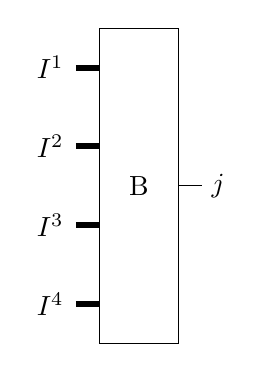
\begin{tikzpicture}[baseline=3]
        \draw (0,2.5)-- (0,-1.5) -- (1,-1.5)-- (1,2.5) -- cycle;

        \node[draw=none] (x)  at (0.5,0.5) {B};

        \draw[line width=0.75mm] (-0.3,2)  node [left] {$I^1$}  -- (0,2) ;
        \draw[line width=0.75mm] (-0.3,1)  node [left] {$I^2$} -- (0,1);
        \draw[line width=0.75mm] (-0.3,0)  node [left] {$I^3$} -- (0,0);
        \draw[line width=0.75mm] (-0.3,-1)  node [left] {$I^4$} -- (0,-1);

        \draw (1,0.5) -- (1.3,0.5)  node [right] {$j$} ;

    \end{tikzpicture} }

An example of this procedure is
\begin{align}
    \pepoat                    & =  \nonumber                                      \\
    \blockat                   &                                                   \\
    \vcenter{\hbox{ \pepoct }} & =\vcenter{\hbox{  \blockct }} . \label{extract_x}
\end{align}

\subsubsection{Linear Solver}

Full inverse
Sequential inverse
Sparse full inverse

\subsubsection{Nonlinear Solver}

\subsubsection{Sequential Solver}

\section{Results}
\subsection{Direct}

%\todo{norm}

\begin{figure*}[h!]
    \center
    \includegraphics[width=0.8\textwidth]{../Figuren/benchmarking/t_ising.pdf}
    \caption{Comparison type A, E and F for Transversal Ising. 1D }
    \label{fig:benchmark:tising}
\end{figure*}

%\todo{heis, 2D, rt}

\subsection{2D Transversal Ising}

\begin{itemize}
    \item g=0 value
    \item g=2.5 value
    \item tricrit
\end{itemize}

\begin{figure*}[h!]
    \center
    \includegraphics[width=\textwidth]{../Figuren/phasediag/g25/zoomed.pdf}
    \caption{ Data collapse for $g=2.5$ phase transition of transversal Ising Model. Data points are taken from $T \in \left[ T_c -0.08, T_c +0.08 \right]$. }
    \label{fig:phase:g25:zoomed}
\end{figure*}

\section{Outlook}

\bibliographystyle{plain}
\bibliography{../bib.bib}
\end{document}
